%%%%%%%%%%%%%%%%%%%%%%%%%%%%%%%%%%%%%%%%%%%%%%%%%%%%%%%%%%%%%%%%%%%%%%%%
% Plantilla TFG/TFM
% Universidad de Murcia. Facultad de Informática
% Realizado por: José Manuel Requena Plens
% Modificado: Pablo José Rocamora Zamora
% Contacto: pablojoserocamora@gmail.com
%%%%%%%%%%%%%%%%%%%%%%%%%%%%%%%%%%%%%%%%%%%%%%%%%%%%%%%%%%%%%%%%%%%%%%%%

\chapter{Anexo}

\begin{table}[h]
\centering
\label{tab:proteinas}
\begin{tabular}{lcccc}
\toprule
\textbf{Proteína} & \textbf{Dimensiones} & \textbf{Volumen total} & \textbf{Vóxels ocupados} & \textbf{Ocupancia interna} \\
    \midrule
    4v4r\_10A & $66 \times 66 \times 66$ & 287\,496 & 5\,440 & 1.89\,\% \\
    5mrc\_10A & $72 \times 72 \times 72$ & 373\,248 & 7\,599 & 2.04\,\% \\
    2uv8\_10A & $48 \times 48 \times 48$ & 110\,592 & 7\,458 & 6.74\,\% \\
    4v94\_10A & $72 \times 72 \times 72$ & 373\,248 & 4\,985 & 1.34\,\% \\
    4cr2\_10A & $66 \times 66 \times 66$ & 287\,496 & 3\,499 & 1.22\,\% \\
    3d2f\_10A & $62 \times 62 \times 62$ & 238\,328 &    739 & 0.31\,\% \\
    3cf3\_10A & $54 \times 54 \times 54$ & 157\,464 &    814 & 0.52\,\% \\
    2cg9\_10A & $52 \times 52 \times 52$ & 140\,608 &    576 & 0.41\,\% \\
    1u6g\_10A & $56 \times 56 \times 56$ & 175\,616 &    741 & 0.42\,\% \\
    1s3x\_10A & $46 \times 46 \times 46$ &  97\,336 &    156 & 0.16\,\% \\
    1qvr\_10A & $56 \times 56 \times 56$ & 175\,616 &    957 & 0.54\,\% \\
    \bottomrule
\end{tabular}
\caption{Proteínas utilizadas en los experimentos (resolución 10\,\AA).}
\end{table}


\begin{figure}[H]
    \centering
    \begin{subfigure}[b]{0.36\textwidth}
        \centering
        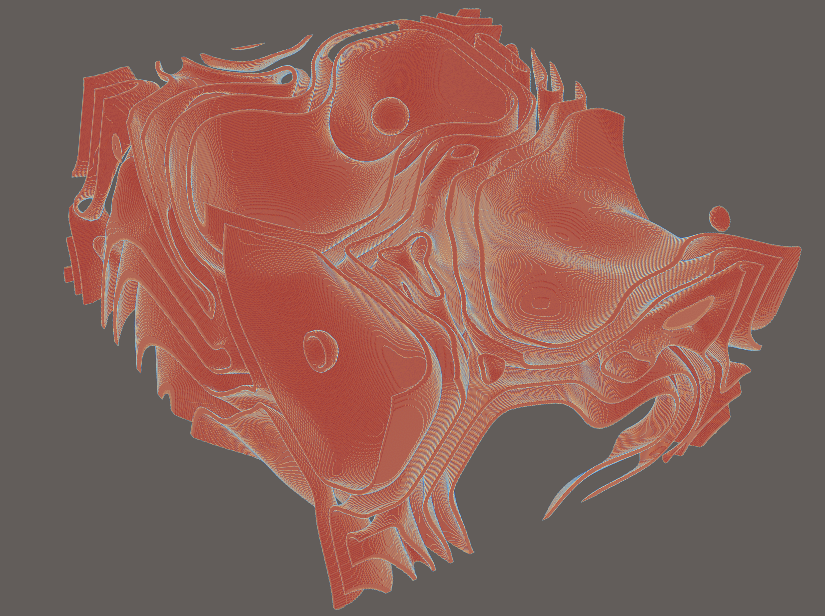
\includegraphics[width=\textwidth]{archivos/membrana0.png}
        \caption{Ocupancia base de 12.88\%}
    \end{subfigure}
     \hspace{0.04\textwidth}
    \begin{subfigure}[b]{0.36\textwidth}
        \centering
        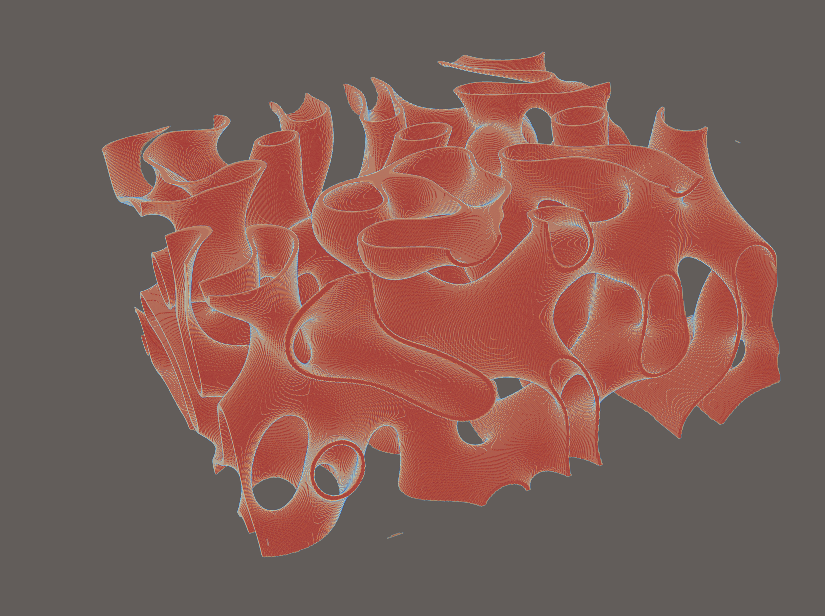
\includegraphics[width=\textwidth]{archivos/membrana1.png}
        \caption{Ocupancia base de 7.43\%}
    \end{subfigure}
    
    \begin{subfigure}[b]{0.36\textwidth}
        \centering
        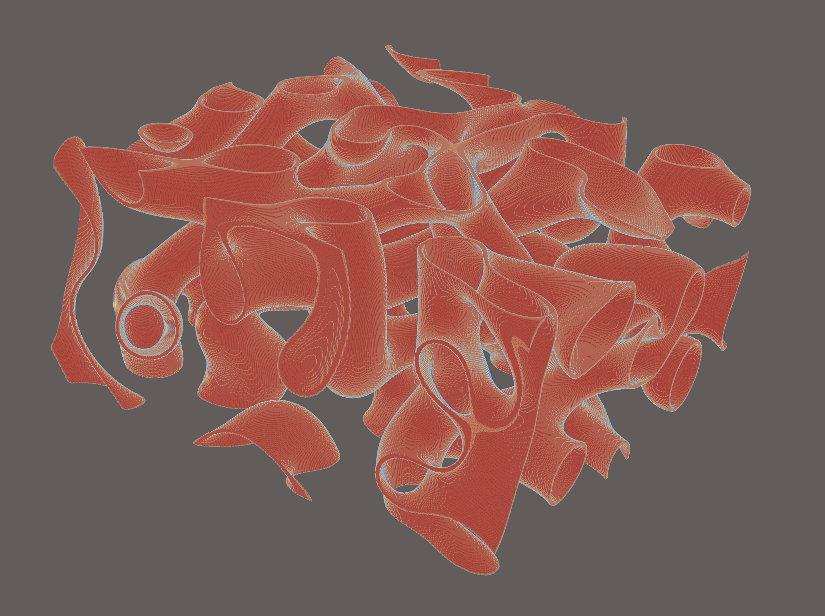
\includegraphics[width=\textwidth]{archivos/membrana2.png}
        \caption{Ocupancia base de 6.63\%}
    \end{subfigure}
     \hspace{0.04\textwidth}
    \begin{subfigure}[b]{0.36\textwidth}
        \centering
        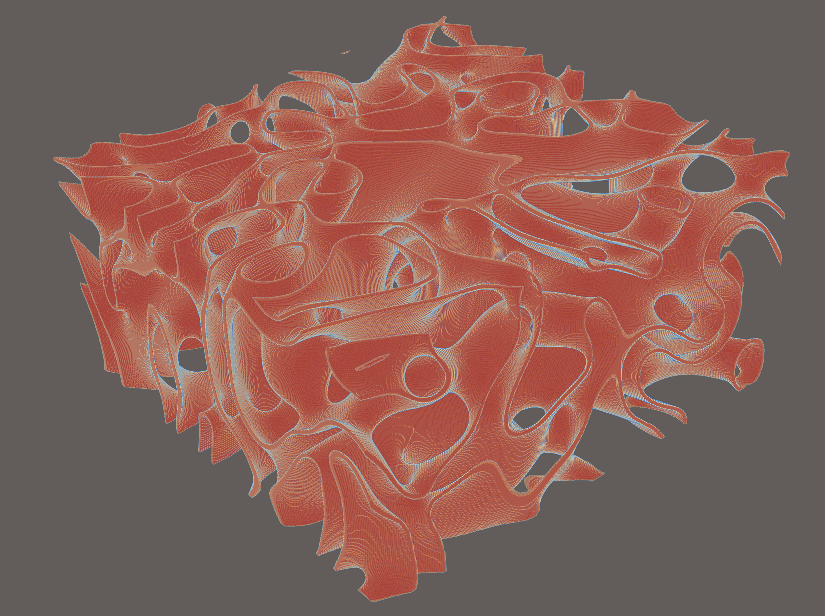
\includegraphics[width=\textwidth]{archivos/membrana3.png}
        \caption{Ocupancia base de 11.54\%}
    \end{subfigure}
    \caption{Membranas sintéticas utilizadas en los experimentos.}
    \label{fig:membranas}
\end{figure}

\begin{figure}[H]
    \centering
    \captionsetup[subfigure]{labelformat=empty}
    \begin{subfigure}[b]{0.36\textwidth}
        \centering
        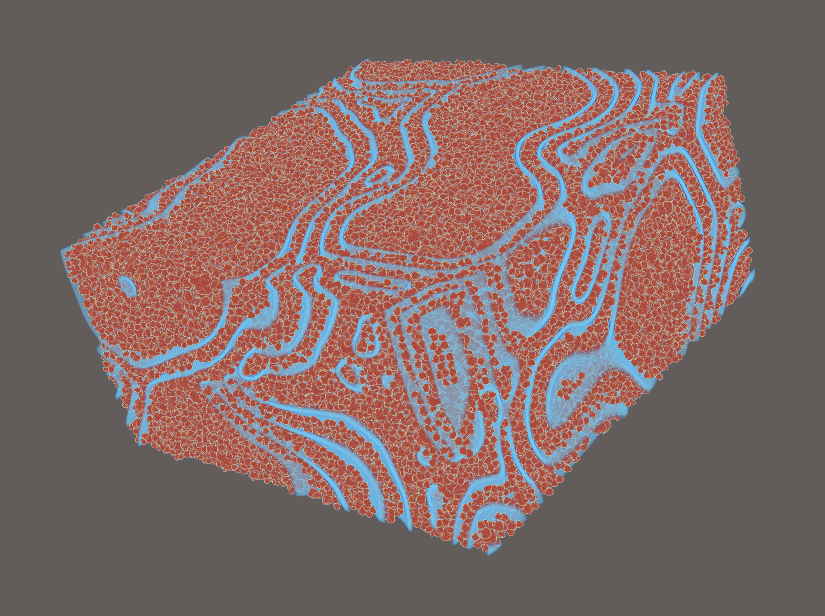
\includegraphics[width=\textwidth]{archivos/tomo0.png}
        \caption{Membrana \textbf{a)}: proteínas 39.25\%, total 52.13\%}
    \end{subfigure}
    \hspace{0.04\textwidth}
    \begin{subfigure}[b]{0.36\textwidth}
        \centering
        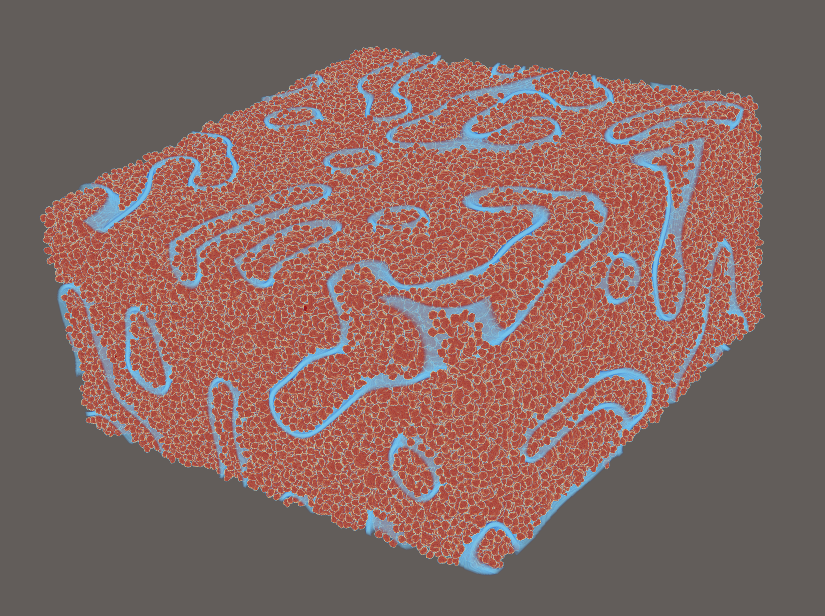
\includegraphics[width=\textwidth]{archivos/tomo1.png}
        \caption{Membrana \textbf{b)}: proteínas 46.55\%, total 53.99\%}
    \end{subfigure}

    \begin{subfigure}[b]{0.36\textwidth}
        \centering
        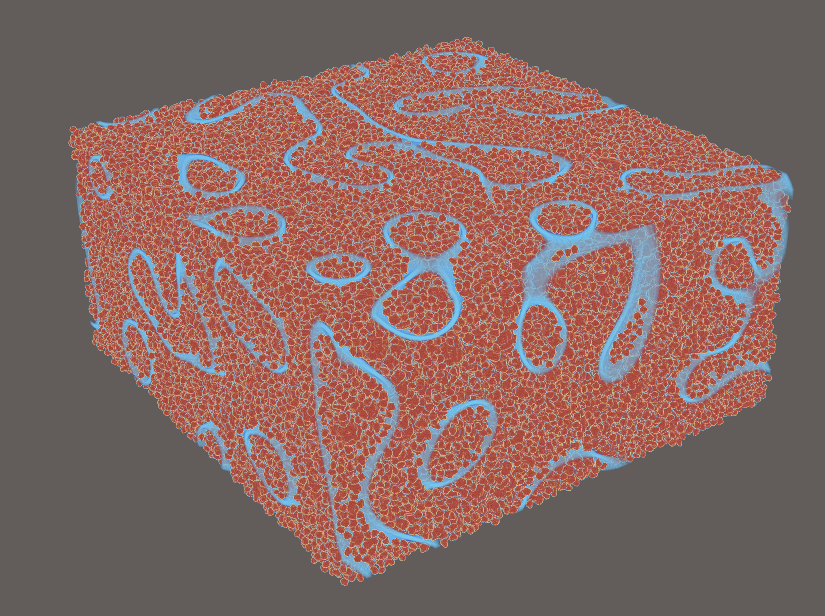
\includegraphics[width=\textwidth]{archivos/tomo2.png}
        \caption{Membrana \textbf{c)}: proteínas 47.62\%, total 54.25\%}
    \end{subfigure}
    \hspace{0.04\textwidth}
    \begin{subfigure}[b]{0.36\textwidth}
        \centering
        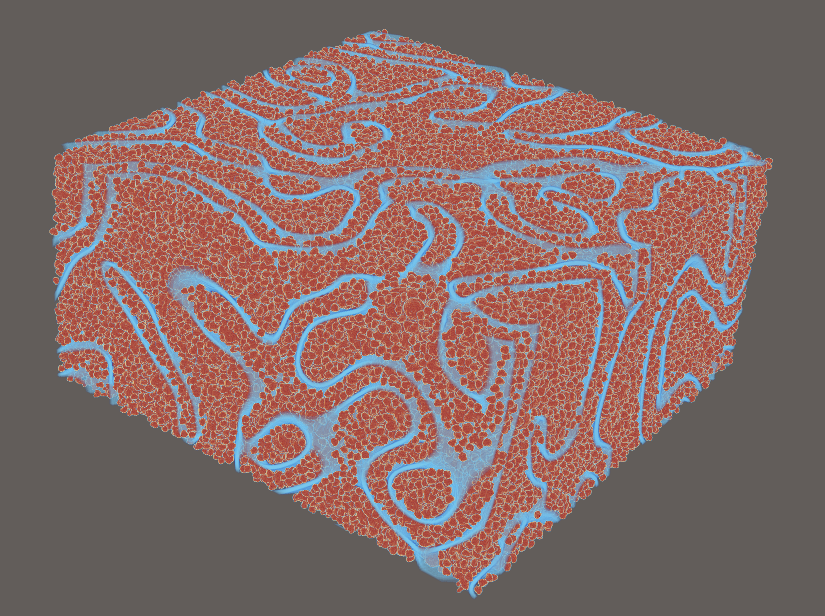
\includegraphics[width=\textwidth]{archivos/tomo3.png}
        \caption{Membrana \textbf{d)}: proteínas 41.65\%, total 53.19\%}
    \end{subfigure}
    \caption{Tomogramas sintéticos generados con Tetris para cada membrana.}
    \label{fig:tomos}
\end{figure}


\begin{table}[h]
\centering
\begin{tabular}{lrrrr}
\toprule
\textbf{Proteína} & \textbf{Membrana a)} & \textbf{Membrana b)} & \textbf{Membrana c)} & \textbf{Membrana d)} \\
\midrule
2uv8\_10A &    777  & 1\,805 & 1\,883 & 1\,140 \\
5mrc\_10A &     52  &    15  &    23  &    44  \\
4v4r\_10A &    155  &   212  &   230  &   137  \\
4v94\_10A &    111  &    98  &    41  &   230  \\
4cr2\_10A &    176  &   324  &   319  &   390  \\
1qvr\_10A &  7\,876 & 3\,981 & 3\,912 & 5\,268 \\
3cf3\_10A &  1\,234 & 1\,078 & 1\,404 & 1\,056 \\
1u6g\_10A &    567  &   635  &   211  &   417  \\
2cg9\_10A &    928  & 1\,428 & 1\,938 & 1\,510 \\
3d2f\_10A &     51  &     0  &     1  &     0  \\
1s3x\_10A & 31\,716 & 29\,812 & 29\,822 & 31\,657 \\
\midrule
\textbf{Total} & \textbf{43\,643} & \textbf{39\,388} & \textbf{39\,784} & \textbf{41\,849} \\
\bottomrule
\end{tabular}
\caption{Número de monómeros insertados por tipo de proteína en cada membrana usando Tetris.}
\label{tab:monomeros}
\end{table}


\begin{figure}[H]
    \centering
    \captionsetup[subfigure]{labelformat=empty}
    \begin{subfigure}[b]{0.36\textwidth}
        \centering
        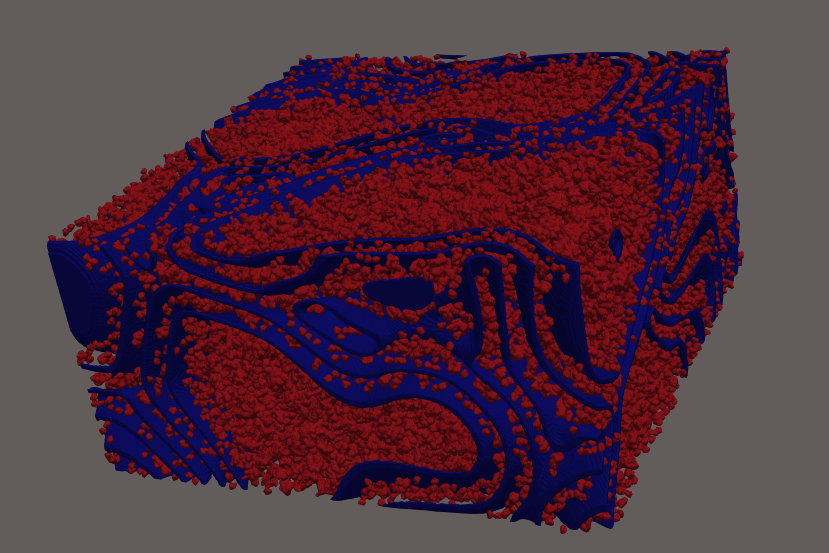
\includegraphics[width=\textwidth]{archivos/tomo_0-sawlc.png}
        \caption{Membrana \textbf{a)}: proteínas 18.63\%, total 31.51\%}
    \end{subfigure}
    \hspace{0.04\textwidth}
    \begin{subfigure}[b]{0.36\textwidth}
        \centering
        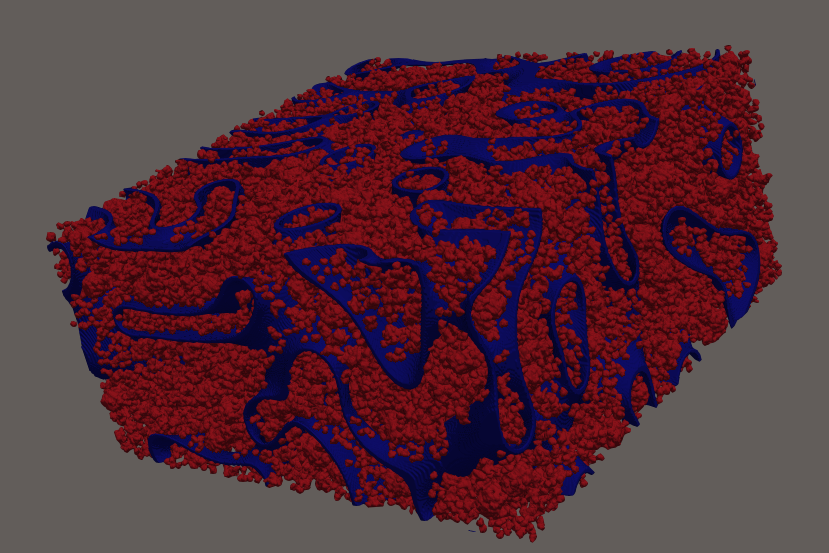
\includegraphics[width=\textwidth]{archivos/tomo_1-sawcl.png}
        \caption{Membrana \textbf{b)}: proteínas 23.66\%, total 31.10\%}
    \end{subfigure}

    \begin{subfigure}[b]{0.36\textwidth}
        \centering
        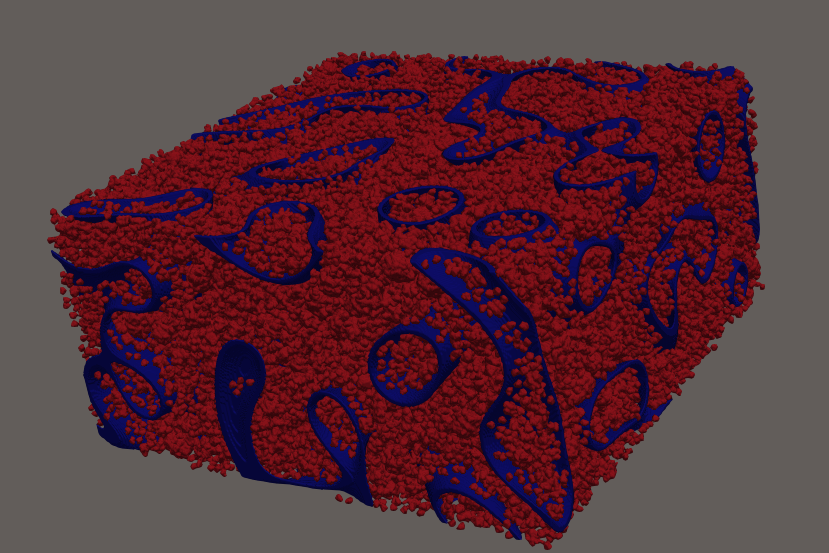
\includegraphics[width=\textwidth]{archivos/tomo_2-sawlc.png}
        \caption{Membrana \textbf{c)}: proteínas 27.08\%, total 33.71\%}
    \end{subfigure}
    \hspace{0.04\textwidth}
    \begin{subfigure}[b]{0.36\textwidth}
        \centering
        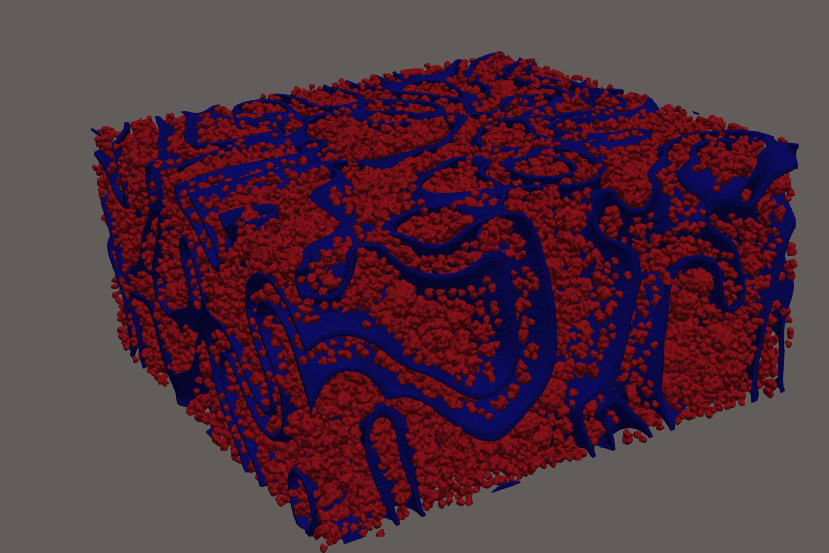
\includegraphics[width=\textwidth]{archivos/tomo_3-sawlc.png}
        \caption{Membrana \textbf{d)}: proteínas 20.17\%, total 31.72\%}
    \end{subfigure}
    \caption{Tomogramas sintéticos generados con SAWLC para cada membrana.}
    \label{fig:tomos-sawlc}
\end{figure}

\begin{table}[h]
\centering
\begin{tabular}{lrrrr}
\toprule
\textbf{Proteína} & \textbf{Membrana a)} & \textbf{Membrana b)} & \textbf{Membrana c)} & \textbf{Membrana d)} \\
\midrule
2uv8\_10A &    362  &    946  & 1\,052 &    446  \\
5mrc\_10A &      3  &      9  &     10 &     14  \\
4v4r\_10A &     45  &     60  &     57 &     86  \\
4v94\_10A &      7  &      0  &     41 &      9  \\
4cr2\_10A &    137  &    168  &     72 &    208  \\
1qvr\_10A &  1\,816 &  2\,836 & 2\,773 &  3\,059 \\
3cf3\_10A &  2\,119 &  1\,103 & 1\,632 &  1\,178 \\
1u6g\_10A &    873  &    287  &    116 &    401  \\
2cg9\_10A &  1\,781 &    409  & 1\,544 &  1\,642 \\
3d2f\_10A &     88  &     20  &     14 &     20  \\
1s3x\_10A & 23\,993 & 23\,159 & 27\,953 & 23\,231 \\
\midrule
\textbf{Total} & \textbf{31\,224} & \textbf{28\,997} & \textbf{35\,264} & \textbf{30\,294} \\
\bottomrule
\end{tabular}
\caption{Número de monómeros insertados por tipo de proteína en cada membrana usando SAWLC.}
\label{tab:monomeros-sawlc}
\end{table}